\chapter{Model grafowy problemu zakupu licencji} \label{ch:graph_model}

Niniejszy rozdział formalizuje analizowany problem, zaczynając od zdefiniowania reprezentacji sieci społecznej, a następnie opisując parametry i ograniczenia wynikające z praktyki licencjonowania. Stanowi to fundament dla późniejszych rozdziałów poświęconych teorii dominowania oraz konstrukcji algorytmów.

\section{Reprezentacja grafowa} 

Aby formalnie opisać zjawisko współdzielenia licencji, sieć relacji społecznych modeluje się jako graf nieskierowany \( G = (V, E) \). Każdy wierzchołek \( v \in V \) reprezentuje pojedynczego użytkownika, natomiast krawędź \( \{u, v\} \in E \) oznacza, że użytkownicy \( u \) i \( v \) znajdują się w relacji umożliwiającej współdzielenie licencji grupowej. Graf jest nieskierowany, ponieważ relacja znajomości jest symetryczna.

Przyjmuje się również, że graf \( G \) nie zawiera pętli ani krawędzi wielokrotnych -- każda para użytkowników może być powiązana co najwyżej jedną krawędzią. Przykład takiej struktury zilustrowano na rysunku~\ref{fig:social_graph}.

\begin{figure}[H]
  \centering
  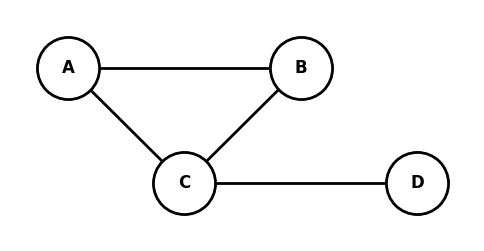
\includegraphics[width=0.5\textwidth]{assets/graphmodelexample.png}
  \caption{Przykładowy graf relacji społecznych między użytkownikami.}
  \label{fig:social_graph}
\end{figure}

Opisana reprezentacja, w której wierzchołki odpowiadają jednostkom, a krawędzie bezpośrednim relacjom umożliwiającym interakcję, jest powszechnie stosowana w analizie sieci społecznościowych \cite{Brandes2005, NETTLETON20131}. Takie ujęcie pozwala formalnie modelować i badać zjawiska zachodzące w społecznościach użytkowników usług cyfrowych.

W przyjętym modelu zakłada się, że współdzielenie licencji może odbywać się wyłącznie między osobami połączonymi bezpośrednią krawędzią w grafie. Licencja grupowa oznacza w tym kontekście typ umożliwiający współdzielenie dostępu przez właściciela oraz jego bezpośrednich sąsiadów. Warunek sąsiedztwa odzwierciedla wymóg bezpośredniej relacji. Zagadnienia zaufania i uwierzytelniania nie są modelowane. Relacje pośrednie, w których użytkownicy są powiązani poprzez wspólnych znajomych (np. \( A \sim B \) oraz \( B \sim C \), lecz brak bezpośredniego powiązania \( A \sim C \)), nie są uwzględniane w analizie. Oznacza to, że dla danego grafu \( G = (V, E) \),
w którym \( V \) to zbiór użytkowników, a \( E \subseteq \{ \{u,v\} : u,v \in V, u \neq v \} \) to zbiór relacji znajomości, analizie podlegają wyłącznie relacje bezpośrednie, czyli pary \( \{u, v\} \in E \).
W grafie z rysunku~\ref{fig:social_graph} użytkownicy \( A \) i \( D \) są połączeni ścieżką \( A \rightarrow C \rightarrow D \), lecz brak krawędzi \( \{A,D\} \in E \) eliminuje możliwość współdzielenia licencji w modelu.
Mimo że w praktyce relacje pośrednie mogą sprzyjać tworzeniu grup, w analizie pominięto je dla uproszczenia problemu.

Graf społecznościowy nie musi być pełny. Dopuszcza się dowolną strukturę odpowiadającą rzeczywistym relacjom społecznym. Istotny jest stopień wierzchołka, gdyż ogranicza liczbę sąsiadów, którym można udostępnić licencję. Dla wierzchołka \( v \in V \), jego stopień oznaczamy przez \( \deg(v) \), co odpowiada liczbie sąsiadów użytkownika \( v \) w grafie \( G = (V, E) \).

Należy jednak zauważyć, że nawet w przypadku wysokiego \( \deg(v) \), użytkownik niekoniecznie może współdzielić licencję ze wszystkimi swoimi sąsiadami. Ograniczenia techniczne, takie jak ograniczenia liczby współużytkowników narzucane przez dostawcę usługi, sprawiają, że liczba osób objętych jedną licencją grupową pozostaje ograniczona. W dalszej części rozdziału omówiono te ograniczenia oraz ich wpływ na model optymalizacji kosztów licencjonowania.


\section{Definicja problemu}\label{sec:model-formal}

Optymalizacja kosztu dostępu do usługi wymaga przypisania wszystkim wierzchołkom grafu $G ~=~ (V,~E)$ odpowiednich ról. Każdy użytkownik $v \in V$ może uzyskać dostęp do usługi na trzy sposoby:
\begin{enumerate}
  \item Poprzez wykupienie licencji indywidualnej.
  \item Poprzez wykupienie licencji grupowej.
  \item Jako odbiorca, korzystający z licencji grupowej należącej do innego użytkownika.
\end{enumerate}
Licencja indywidualna zapewnia dostęp wyłącznie jej właścicielowi, natomiast licencja grupowa umożliwia współdzielenie dostępu z maksymalnie $k-1$ sąsiadami w grafie. Należy przy tym podkreślić, że pojedynczy użytkownik może posiadać najwyżej jedną licencję grupową, nawet jeśli liczba jego sąsiadów przekracza dopuszczalny limit.
Ograniczenie to odzwierciedla typowe postanowienia regulaminowe usługodawców, takie jak powiązanie konta z jednym numerem telefonu oraz limit liczby współużytkowników.
Dla uproszczenia przyjmuje się, że zasada ta obowiązuje wszystkie typy licencji, niezależnie od rzeczywistych warunków oferowanych przez poszczególnych dostawców usług.

Dla przejrzystego i precyzyjnego zdefiniowania modelu wprowadzamy trzy zbiory reprezentujące użytkowników, czyli węzły posiadające własną licencję bądź korzystające z licencji innego węzła:
\begin{itemize}
  \item $I$ - posiadacze licencji indywidualnych;
  \item $H$ - posiadacze licencji grupowych;
  \item $R$ - odbiorcy, którzy sami nie kupują licencji, lecz korzystają z licencji innego użytkownika.
\end{itemize}

Aby formalnie opisać ten podział, wprowadzamy etykietowanie ról $f:V\to\{0,1,2\}$.
Wartość $0$ oznacza węzeł będący odbiorcą, $1$ odpowiada licencji indywidualnej, a $2$ licencji grupowej.
Takie przypisanie nawiązuje do klasycznego problemu dominowania rzymskiego, w którym wierzchołki również otrzymują etykiety z tego samego zbioru wartości.
Odpowiadające zbiory definiujemy jako $I=\{v:f(v)=1\}$, $H=\{v:f(v)=2\}$ oraz $R=V\setminus(I\cup H)$.
Przyjmujemy zbiór dostępnych typów licencji
\begin{equation}
  L = \{ l_t = (c_t, m_t, k_t) \mid t = 1,2,\dots,T \},
  \label{eq:license_family}
\end{equation}
gdzie:
\begin{itemize}
  \item $c_t$ - koszt licencji typu $t$,
  \item $m_t$ - minimalna liczba użytkowników wliczając właściciela,
  \item $k_t$ - maksymalna liczba użytkowników wliczając właściciela,
  \item $T$ - całkowita liczba dostępnych typów licencji.
\end{itemize}

Dla potrzeb jednolitego formalnego opisu w pracy stosowane są wymiennie pojęcia konfiguracja licencyjna, wariant licencyjny oraz schemat licencjonowania, które odnoszą się do konkretnego zbioru typów licencji definiowanego przez $L$. Na przykład Duolingo Super stanowi schemat licencjonowania składający się z dwóch typów licencji: indywidualnej oraz rodzinnej. Analogicznie, dla celów teoretycznych, dominowanie rzymskie traktowane jest jako schemat licencjonowania zawierający licencję indywidualną i grupową. Takie podejście umożliwia sprowadzenie różnych modeli licencjonowania do jednej spójnej abstrakcji matematycznej i ułatwia porównanie wyników między wariantami rzeczywistymi a teoretycznymi.

W podstawowym wariancie rozważanym w tym rozdziale zakładamy, że zbiór $L$ opisany we wzorze~(\ref{eq:license_family}) obejmuje wyłącznie dwa typy licencji: indywidualną oraz jedną grupową, a zatem przyjęte jest $T = 2$. Model ten nie przewiduje sytuacji z wieloma rodzajami planów grupowych (np. Duo, Family), lecz ogranicza się do najprostszego przypadku odpowiadającego rozwiązaniom takim jak w Duolingo.

\paragraph{Warunki wykonalności.}
Spełnienie rozwiązania wymaga, aby dla etykietowania $f:V\to\{0,1,2\}$ zachodziły następujące warunki:
\begin{enumerate}
  \item Pokrycie: Każdy użytkownik $v \in V$ musi mieć dostęp do usługi, tj. $f(v)\in\{1,2\}$ lub istnieje sąsiad $u\in N(v)$ taki, że $f(u)=2$ i $v$ jest przypisany do grupy $u$.
  \item Sąsiedztwo: Odbiorca $v\in R$ może być przypisany tylko do właściciela $u\in H$ z $\{u,v\}\in E$.
  \item Pojemność: Liczba użytkowników przypisanych do właściciela $u\in H$ (wraz z nim samym) musi spełniać $m \le 1+|R_u| \le k$, gdzie $R_u$ oznacza zbiór odbiorców korzystających z licencji $u$.
  \item Jednoznaczność etykiety: każdy wierzchołek $v\in V$ otrzymuje dokładnie jedną etykietę $f(v)\in\{0,1,2\}$.
\end{enumerate}


\paragraph{Funkcja kosztu.}
W wariancie podstawowym, w którym $T=2$, całkowity koszt rozwiązania wyraża się zależnością:
\begin{equation}
  \cost(f) = |I|\cdot c_i + |H|\cdot c_g ,
  \label{eq:cost_function}
\end{equation}
gdzie:
\begin{itemize}
  \item $I$ - zbiór użytkowników z licencją indywidualną,
  \item $H$ - zbiór użytkowników z licencją grupową,
  \item $c_i$ - koszt licencji indywidualnej,
  \item $c_g$ - koszt licencji grupowej.
\end{itemize}

\paragraph{Cel optymalizacji.}
Celem problemu jest minimalizacja funkcji kosztu~(\ref{eq:cost_function}) dla danego grafu $G=(V,E)$, przy spełnieniu wszystkich istotnych warunków wykonalności.


\section{Koszty i ograniczenia} \label{sec:costs_constraints}

W tej części zestawiono parametry, które przekładają się na realną wykonalność i opłacalność grup licencyjnych. Najpierw omówiono ograniczenia pojemności wynikające z regulaminów usług, a następnie struktury cenowe wykorzystywane później w eksperymentach.

\subsection{Ograniczenia techniczne i społeczne współdzielenia licencji}

Kluczowymi parametrami modelu są najmniejsza oraz największa liczba osób, które mogą współdzielić jedną licencję grupową. Największy rozmiar grupy oznaczamy przez $k$ i wliczamy do niego także użytkownika nabywającego licencję. Parametr $k$ jest zwykle narzucany przez dostawcę usługi. Przykładowo, plan rodzinny Spotify Premium pozwala na korzystanie co najwyżej sześciu osobom (właściciel + pięć członków rodziny), co odpowiada wartości $k=6$.

Analogicznie wprowadzamy parametr $m$, który określa najmniejszą liczbę osób niezbędnych do utworzenia grupy. Oznacza to, że licencja grupowa jest ważna tylko wtedy, gdy zostanie wykorzystana przez co najmniej $m$ osób (łącznie z właścicielem). Przykładem jest plan "Duo", w którym licencję współdzielą dokładnie dwie osoby ($m=2, k=2$). W innych przypadkach $m$ może przyjmować wartości mniejsze niż $k$, np. $m=2, k=6$ dla planów rodzinnych.

W analizie przyjmujemy $m$ oraz $k$ jako zmienne parametry. Nawet jeśli użytkownik posiada wielu znajomych (czyli ma wysoki stopień w grafie), ograniczenie $k$ sprawia, że może objąć współdzieleniem tylko określoną najwyższą liczbę osób, natomiast ograniczenie $m$ wymusza, by grupy nie były zbyt małe. Parametry te modelują zarówno ograniczenia techniczne narzucane przez dostawców usług, jak i czynniki społeczne, takie jak opłacalność czy gotowość do współdzielenia subskrypcji. W konsekwencji grupy współdzielenia odwzorowują typowe sytuacje, w których w praktyce licencje grupowe są wykorzystywane.

\subsection{Struktura kosztów i modele cenowe}

W analizowanym problemie istotnym elementem jest sposób odwzorowania polityki cenowej dostawców usług.
Różne plany subskrypcyjne charakteryzują się nie tylko innym kosztem, ale również odmiennym zakresem liczby użytkowników $m$ oraz $k$, którzy mogą korzystać z jednej licencji.
Rodzinę typów licencji zdefiniowaną we wzorze~\eqref{eq:license_family} stosujemy tutaj do opisu struktury kosztów i ograniczeń dostępnych planów.
W testach syntetycznych wartości parametrów licencji dobierane są eksperymentalnie, co pozwala badać zachowanie algorytmów w różnych wariantach cenowych i strukturalnych.
W testach na danych rzeczywistych wykorzystywane są faktyczne ceny subskrypcji.
Dla wariantu teoretycznego odpowiadającego dominowaniu rzymskiemu koszty normalizowane są względem licencji indywidualnej, co umożliwia powiązanie modelu z klasycznymi zagadnieniami teorii grafów.
Przykłady zestawiono w~tabeli~\ref{tab:license_models_real}.


\begin{table}[h!]
  \centering
  \caption{Przykładowe schematy licencjonowania dla usług rzeczywistych i modelu teoretycznego.}
  \begin{tabular}{lccc}
    \hline
    \textbf{Typ licencji} & \textbf{Koszt $c_t$} & \textbf{Min $m_t$} & \textbf{Max $k_t$} \\
    \hline
    \multicolumn{4}{c}{\textit{Spotify (ceny w PLN)}}                                      \\
    Individual            & 23.99                & 1                  & 1                  \\
    Duo                   & 30.99                & 2                  & 2                  \\
    Family                & 37.99                & 2                  & 6                  \\
    \hline
    \multicolumn{4}{c}{\textit{Netflix (ceny w PLN)}}                                      \\
    Basic                 & 33.00                & 1                  & 1                  \\
    Standard              & 49.00                & 1                  & 2                  \\
    Premium               & 67.00                & 1                  & 4                  \\
    \hline
    \multicolumn{4}{c}{\textit{Duolingo Super (ceny w PLN)}}                               \\
    Individual            & 13.99                & 1                  & 1                  \\
    Family                & 29.17                & 2                  & 6                  \\
    \hline
    \multicolumn{4}{c}{\textit{Model teoretyczny (koszty znormalizowane)}}                 \\
    Solo                  & 1.0                  & 1                  & 1                  \\
    Group                 & 2.0                  & 2                  & 999999             \\
    \hline
    \label{tab:license_models_real}
  \end{tabular}

  Źródło: opracowanie własne modelu teoretycznego oraz \cite{spotify_price2025}, \cite{netflix_price2025}, \cite{duolingo_app2024}.

\end{table}


W przypadku usług rzeczywistych koszty planów grupowych są znacznie niższe niż suma odpowiadających im licencji indywidualnych. Przykładowo plan Spotify Family dopuszcza współdzielenie przez co najwyżej sześć osób przy koszcie $37.99$ PLN, co jest korzystniejsze kosztowo niż plan indywidualny ($23.99$ PLN). Podobna sytuacja występuje w przypadku Duolingo Super Family.

W modelu teoretycznym opartym na dominowaniu rzymskim koszty podano w jednostkach względnych: licencja indywidualna ma koszt $1.0$, a grupowa $2.0$. W dalszych rozdziałach będziemy odnosić się do tego wariantu jako do schematu licencjonowania dominowania rzymskiego (lub równoważnie konfiguracji licencyjnej lub wariant licencyjny), traktując go jako sformalizowany odpowiednik rzeczywistych planów subskrypcyjnych. Konstrukcja ta spełnia kryteria wykonalności zgodne z zasadami dominowania rzymskiego, a jedyną różnicą pozostaje brak istotnego ograniczenia pojemności -- w klasycznym ujęciu wierzchołek z etykietą 2 może pokrywać dowolnie wielu sąsiadów, co odpowiada planowi grupowemu z praktycznie nieograniczoną liczbą użytkowników. Zgodnie jednak z tabelą \ref{tab:license_models_real}, w implementacji przyjęto duży, ale skończony limit równy 999999. W ramach przeprowadzanych eksperymentów etykieta 2 będzie zmieniała swoją wartość jako wielokrotność kosztu ceny indywidualnej, co pozwala na analizę różnych wariantów tego zagadnienia. W eksperymentach rozważa się także warianty, w których koszt odpowiadający etykiecie \(2\) stanowi wielokrotność kosztu licencji indywidualnej.


\subsection{Zakup jednoczesny i sekwencyjny}

W najprostszym wariancie zakłada się, że wszystkie decyzje zakupowe zapadają w tym samym momencie. Umożliwia to globalną optymalizację i stanowi punkt odniesienia dla analiz teoretycznych. W praktyce jednak proces współdzielenia licencji jest bardziej dynamiczny. Użytkownicy dołączają do planów w różnych momentach; część początkowo wybiera licencje indywidualne, a następnie przechodzi na licencje grupowe. Takie zmiany mogą wynikać z równoczesnej ewolucji struktury sieci społecznościowej. Relacje mogą zanikać, pojawiać się nowe połączenia, a liczba aktywnych użytkowników może się zmieniać.

Takie sytuacje można modelować jako proces sekwencyjny, w którym w kolejnych krokach przydzielane są nowe licencje przy uwzględnieniu bieżącej struktury grafu. W konsekwencji problem różni się od wariantu jednoczesnego. Rozwiązanie optymalne globalnie może okazać się nieosiągalne, ponieważ wcześniejsze decyzje oraz zmiany w strukturze sieci ograniczają przestrzeń dostępnych opcji w późniejszych etapach.

W pracy przeanalizowano konsekwencje takich zmian, w tym stabilność utworzonych grup, wpływ zmian w grafie na opłacalność wcześniejszych decyzji oraz mechanizmy koordynacji i adaptacji użytkowników. Mimo że główny nacisk położony jest na wariant jednoczesny, wariant sekwencyjny stanowi istotne rozszerzenie modelu i lepiej odzwierciedla rzeczywiste warunki funkcjonowania sieci społecznościowych.

\section{Podsumowanie}

Rozwinięty model opisuje sieć społeczną jako graf, w którym decyzje licencyjne są ograniczone zarówno relacjami sąsiedztwa, jak i parametrami minimalnej oraz maksymalnej pojemności planów. Ujednolicone przedstawienie kosztów i wariantów zakupu pozwala w kolejnych rozdziałach analizować złożoność problemu, zależności z klasycznymi zadaniami dominowania oraz efektywność projektowanych algorytmów.
